\documentclass[../../main/main.tex]{subfiles}
\graphicspath{{./figures/}}
\usepackage{custikz}

\dominitoc
\faketableofcontents

\renewcommand{\mtcSfont}{\small\bfseries}
\renewcommand{\mtcSSfont}{\footnotesize}
\mtcsettitle{minitoc}{}
\mtcsetrules{*}{off}

\makeatletter
\renewcommand{\@chapapp}{Thermodynamique -- chapitre}
\makeatother

% \toggletrue{student}
% \toggletrue{corrige}
% \renewcommand{\mycol}{black}
% \renewcommand{\mycol}{gray}

\hfuzz=5.003pt

\begin{document}
\setcounter{chapter}{3}

\settype{book}
\settype{prof}
\settype{stud}

\chapter{Second principe de la thermodynamique}

\epigraph{\openquote\textit{%
		The law that entropy increases -- the Second Law of Thermodynamics -- holds,
		I think, the supreme position among the laws of Nature.}%
	\closequote}{Arthur \textsc{Eddington},
	\textit{The Nature of the Physical World}, 1928}

\vspace*{\fill}

\begin{tcn}*(appl)<ctc>{\iconsomm~Sommaire}
	\let\item\olditem
	\vspace{-15pt}
	\minitoc
	\vspace{-25pt}
\end{tcn}
\begin{tcn}*[fontupper=\small](appl)<ctb>"how"'t'{Capacités exigibles}
	\begin{itemize}[label=\rcheck]
		\item Interpréter qualitativement l'entropie en termes de désordre
		      statistique à l'aide de la formule de Boltzmann fournie.

		\item Définir un système fermé et établir pour ce système un bilan
		      entropique.

		\item Relier la création d'entropie à une ou plusieurs causes physiques de
		      l'irréversibilité.

		\item Analyser le cas particulier d'un système en évolution adiabatique.

		\item Utiliser l'expression fournie de la fonction d'état entropie.

		\item Exploiter l'extensivité de l'entropie.

		\item Citer et utiliser la loi de Laplace et ses conditions
		      d'application.
	\end{itemize}
\end{tcn}

\vspace*{\fill}

\newpage

\vspace*{\fill}
% {
% \begin{boxes}
\begin{tcn}[sidebyside, fontupper=\small, fontlower=\small](appl)<ctb>"check"'t'{L'essentiel}
	\begin{tcn}(defi)<ctc>'t'{Définitions}
		\tcblistof[\paragraph*]{defi}{\hspace*{4.8pt}}
	\end{tcn}
	% \begin{tcn}(rapp)<ctc>'t'{Rappels}
	% 	\tcblistof[\paragraph*]{rapp}{\hspace*{4.8pt}}
	% \end{tcn}
	\begin{tcn}(prop)<ctc>'t'{Propriétés}
		\tcblistof[\paragraph*]{prop}{\hspace*{4.8pt}}
		\tcblistof[\paragraph*]{loi}{\hspace*{4.8pt}}
		% \tcblistof[\paragraph*]{theo}{\hspace*{4.8pt}}
	\end{tcn}
	% \begin{tcn}(coro)<ctc>'t'{Corollaires}
	%   \tcblistof[\paragraph*]{coro}{\hspace*{4.8pt}}
	% \end{tcn}
	\begin{tcn}(demo)<ctc>'t'{Démonstrations}
		\tcblistof[\paragraph*]{demo}{\hspace*{4.8pt}}
		\tcblistof[\paragraph*]{prev}{\hspace*{4.8pt}}
	\end{tcn}
	\begin{tcn}(inte)<ctc>'t'{Interprétations}
		\tcblistof[\paragraph*]{inte}{\hspace*{4.8pt}}
	\end{tcn}
	% \begin{tcn}(impl)<ctc>'t'{Implications}
	% 	\tcblistof[\paragraph*]{impl}{\hspace*{4.8pt}}
	% \end{tcn}
	% \begin{tcn}(tool)<ctc>'t'{Outils}
	% 	\tcblistof[\paragraph*]{tool}{\hspace*{4.8pt}}
	% \end{tcn}
	% \begin{tcn}(nota)<ctc>'t'{Notations}
	%   \tcblistof[\paragraph*]{nota}{\hspace*{4.8pt}}
	% \end{tcn}
	% \begin{tcn}(appl)<ctc>'t'{Applications}
	%   \tcblistof[\paragraph*]{appl}{\hspace*{4.8pt}}
	% \end{tcn}
	% \begin{tcn}(rema)<ctc>'t'{Remarques}
	%   \tcblistof[\paragraph*]{rema}{\hspace*{4.8pt}}
	% \end{tcn}
	% \begin{tcn}(exem)<ctc>'t'{Exemples}
	%   \tcblistof[\paragraph*]{exem}{\hspace*{4.8pt}}
	% \end{tcn}
	% \begin{tcn}*(ror)<ctc>"hart"'t'{Points importants}
	%   \tcblistof[\paragraph*]{ror}{\hspace*{4.8pt}}
	% \end{tcn}
	% \begin{tcn}(impo)<ctc>'t'{Erreurs communes}
	%   \tcblistof[\paragraph*]{impo}{\hspace*{4.8pt}}
	% \end{tcn}
	\tcblower
	% \begin{tcn}(defi)<ctc>'t'{Définitions}
	%   \tcblistof[\paragraph*]{defi}{\hspace*{4.8pt}}
	% \end{tcn}
	% \begin{tcn}(rapp)<ctc>'t'{Rappels}
	%   \tcblistof[\paragraph*]{rapp}{\hspace*{4.8pt}}
	% \end{tcn}
	% \begin{tcn}(prop)<ctc>'t'{Propriétés}
	%   \tcblistof[\paragraph*]{prop}{\hspace*{4.8pt}}
	%   \tcblistof[\paragraph*]{loi}{\hspace*{4.8pt}}
	%   \tcblistof[\paragraph*]{theo}{\hspace*{4.8pt}}
	% \end{tcn}
	% \begin{tcn}(coro)<ctc>'t'{Corollaires}
	%   \tcblistof[\paragraph*]{coro}{\hspace*{4.8pt}}
	% \end{tcn}
	% \begin{tcn}(demo)<ctc>'t'{Démonstrations}
	% 	\tcblistof[\paragraph*]{demo}{\hspace*{4.8pt}}
	% 	\tcblistof[\paragraph*]{prev}{\hspace*{4.8pt}}
	% \end{tcn}
	% \begin{tcn}(inte)<ctc>'t'{Interprétations}
	% 	\tcblistof[\paragraph*]{inte}{\hspace*{4.8pt}}
	% \end{tcn}
	\begin{tcn}(impl)<ctc>'t'{Implications}
		\tcblistof[\paragraph*]{impl}{\hspace*{4.8pt}}
	\end{tcn}
	% \begin{tcn}(tool)<ctc>'t'{Outils}
	%   \tcblistof[\paragraph*]{tool}{\hspace*{4.8pt}}
	% \end{tcn}
	% \begin{tcn}(nota)<ctc>'t'{Notations}
	%   \tcblistof[\paragraph*]{nota}{\hspace*{4.8pt}}
	% \end{tcn}
	\begin{tcn}(appl)<ctc>'t'{Applications}
		\tcblistof[\paragraph*]{appl}{\hspace*{4.8pt}}
	\end{tcn}
	% \begin{tcn}(rema)<ctc>'t'{Remarques}
	%   \tcblistof[\paragraph*]{rema}{\hspace*{4.8pt}}
	% \end{tcn}
	% \begin{tcn}(exem)<ctc>'t'{Exemples}
	% 	\tcblistof[\paragraph*]{exem}{\hspace*{4.8pt}}
	% \end{tcn}
	\begin{tcn}*(ror)<ctc>"hart"'t'{Points importants}
		\tcblistof[\paragraph*]{ror}{\hspace*{4.8pt}}
	\end{tcn}
	\begin{tcn}(impo)<ctc>'t'{Erreurs communes}
		\tcblistof[\paragraph*]{impo}{\hspace*{4.8pt}}
	\end{tcn}
\end{tcn}
% \end{boxes}
% }%

\vspace*{\fill}
\newpage

\section{L'entropie}

Le premier principe traduit la conservation de l'énergie lors de l'évolution
d'un système. Cependant il ne dit rien sur le sens de cette évolution~: peut–on
toujours retourner de l'état final à l'état initial en passant par le même
chemin~?

La réponse est non~: un système isolé ne peut subir n'importe quelle
transformation ! Un système évoluera toujours d'un état hors équilibre vers un
état d'équilibre, et pas l'inverse.

Ce constat est \textit{a priori} intuitif, puisqu'il décrit l'évolution même du
temps et notre expérience de son écoulement (un verre cassé ne se répare pas
tout seul), mais il est nécessaire de l'introduire mathématiquement.

\subsection{Statistique}
Pour comprendre la notion d'entropie, on doit s'intéresser à la probabilité
qu'un événement physique survienne.

Reprenons l'exemple de la détente de \textsc{Joule Gay-Lussac}\ftn{Pour une
	visualisation animée, voir la simulation de la diffusion de PhET Colorado~:
	\url{https://phet.colorado.edu/sims/html/diffusion/latest/diffusion_all.html}}~:
soit $N$ molécules de gaz confinées dans une enceinte indéformable et athermane
de volume total $V$, séparée en deux volumes égaux par une cloison. Dans l'état
initial, on injecte toutes les particules dans le compartiment de gauche.

\begin{figure}[htbp!]
	\sswitch{
		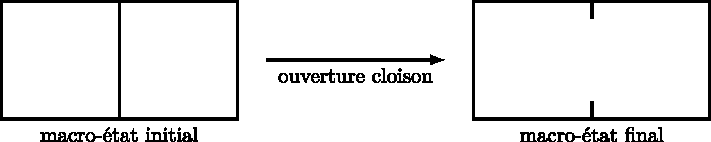
\includegraphics[scale=1]{jgl_intro-stud}
	}{
		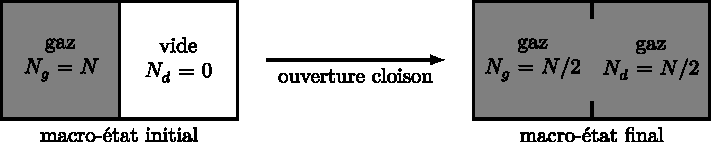
\includegraphics[scale=1]{jgl_intro}
	}
	\caption{Évolution spontanée dans l'expérience de \textsc{Joule Gay-Lussac}}
\end{figure}

On définit les éléments suivants~:
\begin{tcb}(defi){États statistiques d'un système}
	\begin{itemize}
		\item[b]{Micro-état}: \psw{c'est la donnée de l'état de \textbf{chaque}
			particule (vitesse, position)~;}
		\item[b]{Macro-état}: \psw{c'est la donnée des \textbf{grandeurs
				macroscopiques} (pression, température…)}
		\item[b]{Nombre de configurations}: noté $\Omega$, \psw{c'est le nombre de
			\textbf{micro-états compatibles avec un macro-état}.}
	\end{itemize}
\end{tcb}

On s'intéresse alors au nombre de particules dans le compartiment de gauche
$N_g$ et dans le compartiment de droite $N_d$~: ce sont des macro-états, qui
peuvent être réalisés par différents micro-états. Par exemple, pour $N = 2$, il
y a $\Omega\ind{tot} = 4$ micro-états différents, et pour le macro-état $N_g$ il
y en a 3 différents~:

\begin{figure}[htbp!]
	\sswitch{
		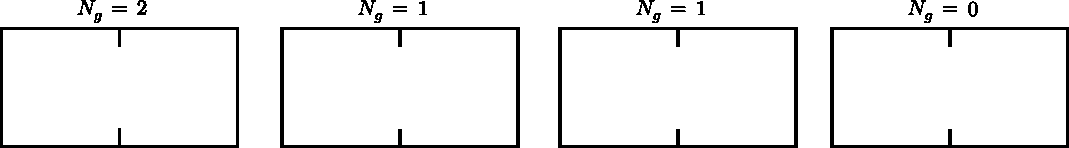
\includegraphics[width=\linewidth]{jgl_n2-stud}
	}{
		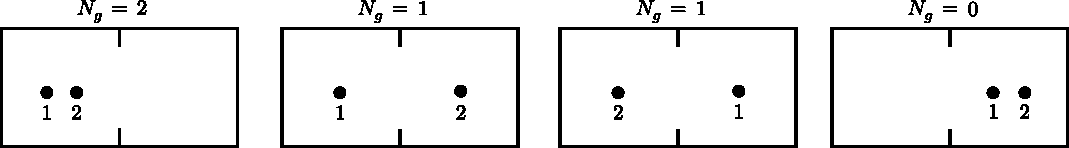
\includegraphics[width=\linewidth]{jgl_n2}
	}
	\vspace{-15pt}
	\caption{Décompte des micro-états pour 2 particules}
\end{figure}

\textbf{Chacun de ces états est possiblement accessible}, mais il apparaît
clairement que l'un d'entre eux est plus \textbf{probable} que les autres~: il y
a deux manières d'arranger les particules pour avoir le macro-état $N_g = 1$,
contre une seule pour les deux autres. On peut remplir le tableau suivant~:

\begin{center}
	\begin{tabular}{ccc}
		\toprule
		\textbf{Macro-état}     &
		\textbf{Configurations} &
		\textbf{Probabilité}
		\\
		\midrule
		$N_g = 0$               &
		\psw{$\Omega = 1$}      &
		$P(N_g = 0) = \psw{\DS\frac{\Omega}{\Omega\ind{tot}} = \num{0.25}}$
		\\
		$N_g = 1$               &
		\psw{$\Omega = 2$}      &
		$P(N_g = 1) = \psw{\DS\frac{\Omega}{\Omega\ind{tot}} = \num{0.50}}$
		\\
		$N_g = 2$               &
		\psw{$\Omega = 1$}      &
		$P(N_g = 2) = \psw{\DS\frac{\Omega}{\Omega\ind{tot}} = \num{0.25}}$
		\\
		\bottomrule
	\end{tabular}
\end{center}

On voit alors apparaître la notion d'entropie et également ce qui définit la
flèche du temps~: les états évoluent vers les \textbf{macro-états les plus
	probables}, c'est-à-dire ceux \textbf{de plus grandes configurations}.

\noindent
\begin{minipage}[c]{.50\linewidth}
	Pour appliquer cette idée à la thermodynamique, il faut l'appliquer à des
	systèmes thermodynamiques, c'est-à-dire comprenant un grand nombre de
	particules. Dans ce cas, $\Omega(N_g)$ se calcule avec\ftn{On retrouve ce
		calcul derrière le triangle de \textsc{Pascal} en mathématiques.}~:
	\[
		\Omega(N_g) =
		\psw{\mqty(N\ind{tot}\\N_g) =
			\frac{N\ind{tot}!}{N_g!(N\ind{tot}-N_g)!}}
	\]
\end{minipage}
\hfill
\begin{minipage}[c]{.48\linewidth}
	\begin{center}
		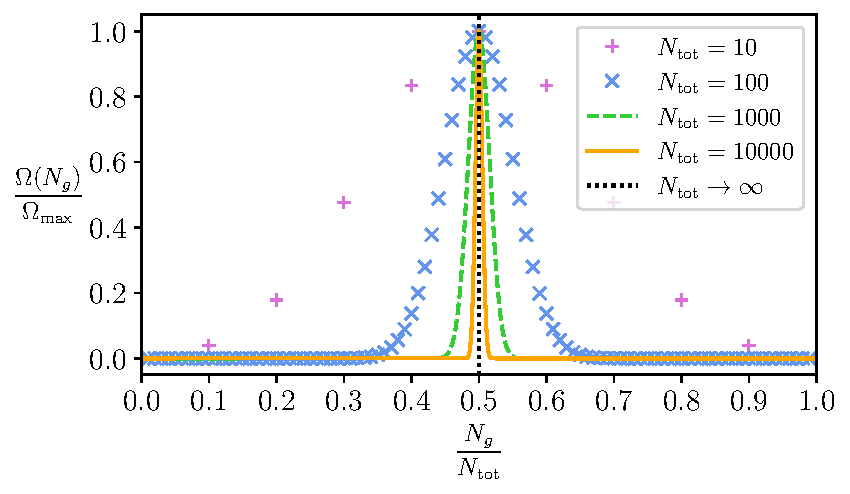
\includegraphics[width=\linewidth]{proba_etat}
	\end{center}
\end{minipage}

Cette distribution est alors \textbf{maximale pour $N_g = N/2$}, c'est-à-dire
$\Omega\ind{max} = \Omega(N/2)$, mais surtout \textbf{décroît exponentiellement
	vite pour $N_g \neq N/2$}.

\begin{tcb*}(defi){Formule de \textsc{Boltzmann}}
	L'entropie d'un système thermodynamique \textbf{isolé} et \textbf{à
		l'équilibre} est une fonction d'état \textbf{extensive} et \textbf{additive},
	donnée par la formule
	\smallbreak
	\begin{isd}
		\vspace{-15pt}
		\psw{%
			\[
				\boxed{S = k_B \ln \Omega}
			\]
		}%
		\vspace{-25pt}
		\tcblower
		\vspace{-15pt}
		\tcbsubtitle{\fatbox{\textbf{Unité}}}
		\psw{%
			\[
				\si{J.K^{-1}}
			\]
		}%
		\vspace{-25pt}
	\end{isd}
	avec $k_B = \SI{1.38e-23}{J.K^{-1}}$ la constante de \textsc{Boltzmann} et
	$\Omega$ le nombre de configurations décrivant le macro-état observé.
\end{tcb*}
\begin{tcb*}(inte){Entropie selon \textsc{Boltzmann}}
	Ainsi, plus $\Omega$ est grand, plus l'entropie est grande~: l'entropie est
	une mesure de la \textbf{probabilité de réalisation} d'un macro-état. Étant
	donné que les états les moins probables sont les plus «~ordonnés~» ($\Omega =
		1$), on dit également que \textbf{l'entropie est une mesure du désordre
		microscopique} d'un système.
	\bigbreak
	Elle \textbf{évolue naturellement vers son augmentation}, et mène à de
	l'irréversibilité~: par un phénomène statistique collectif propre aux systèmes
	de grand nombre de particule, l'évolution vers des états ordonnés est
	\textbf{statistiquement impossible}.
\end{tcb*}

C'est cette idée qui régit l'évolution du gaz de l'état initial à l'état final
dans l'expérience de \textsc{Joule Gaz-Lussac}, mais qui régit également
l'équilibre des températures de deux gaz de températures initialement
différentes. Voir l'animation précédente pour une simulation.

\begin{tcn}*[breakable](exem)<lftt>"yout"{Liens vidéos}
	\begin{tasks}[label=\bdmd](3)
		\task \href{https://www.youtube.com/watch?v=VCXqELB3UPg}{Alpha Phoenix}
		(anglais)
		\task \href{https://www.youtube.com/watch?v=DxL2HoqLbyA}{Veritasium}
		(anglais)
		\task \href{https://www.youtube.com/watch?v=flz_aSIJS0A}{Science Clic}
		(français)
	\end{tasks}
\end{tcn}

\subsection{Irréversibilité}
D'après la section précédente, l'entropie évolue naturellement dans le sens de
son augmentation. C'est pourquoi la mise en contact d'un bloc de cuivre chaud
dans de l'eau donne l'évolution temporelle suivante~:
\begin{figure}[htbp]
	\centering
	\sswitch{
		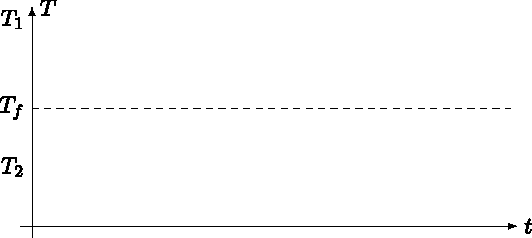
\includegraphics[scale=1]{evol_temp-stud}
	}{
		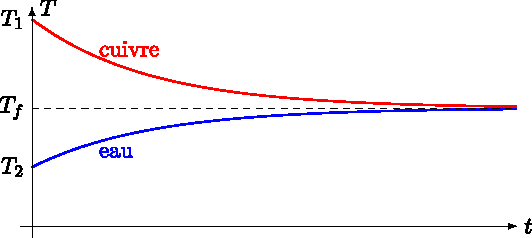
\includegraphics[scale=1]{evol_temp}
	}
\end{figure}

D'une manière générale, deux corps de températures différentes en contact
équilibrent leurs températures~:

\begin{figure}[htbp]
	\centering
	\sswitch{
		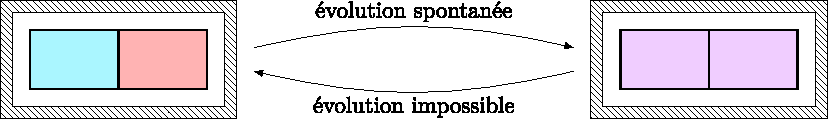
\includegraphics[scale=1]{evol_temp_gen-stud}
	}{
		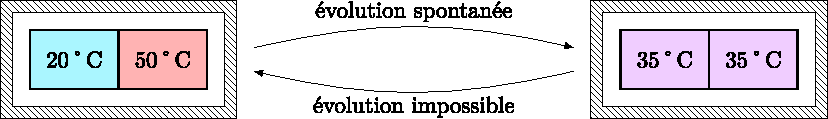
\includegraphics[scale=1]{evol_temp_gen}
	}
\end{figure}

On observe la même chose en mécanique~:

\begin{figure}[htbp]
	\centering
	\sswitch{
		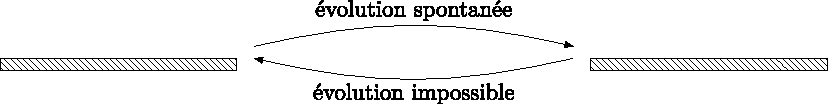
\includegraphics[scale=1]{evol_vits-stud}
	}{
		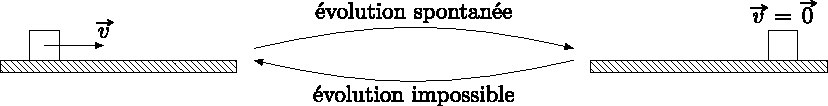
\includegraphics[scale=1]{evol_vits}
	}
\end{figure}

On a alors les critères suivants~:
\begin{tcb*}(prop){Transformations réversibles ou non}
	\begin{itemize}
		\item[b]{Réversible}: une transformation est réversible si
		\begin{itemize}
			\item \psw{elle est \textbf{quasi-statique}, c'est-à-dire en équilibre
				      interne à tout instant~;}
			\item \psw{on peut inverser le sens d'évolution par une
				      \textbf{modification infinitésimale} des paramètres extérieurs}
		\end{itemize}
		\item[b]{Irréversible}:
		\begin{itemize}
			\item le système ne peut \textbf{pas suivre} la transformation en
			      \textbf{sens inverse} en passant par les mêmes états intermédiaires.
			\item les causes~: \psw{toute \textbf{inhomogénéité} interne
				      (température, pression), tous les \textbf{frottements} (transfert
				      d'énergie sous forme de chaleur), et les \textbf{réactions
					      chimiques}.}
		\end{itemize}
	\end{itemize}
\end{tcb*}

\begin{tcb}[breakable](exem)<lftt>{Transformations réversibles ou non}
	\tcbsubtitle{\fatbox{\textbf{Entropie d'une goutte d'encre}}}
	En plaçant une goutte de colorant dans de l'eau, celle-ci se répartit dans
	l'espace disponible, \textbf{sans retour en arrière possible}, ce qui
	s'explique pas les micro-états compatibles avec chaque situation.
	\begin{center}
		\begin{tabularx}{.7\linewidth}{|l|Y|Y|}
			\hline
			                                                &
			\textbf{État initial}                           &
			\textbf{État ultérieur}
			\\\hline
			\rotatebox[origin=c]{90}{Macro-état}            &
			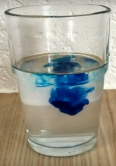
\includegraphics[height=3cm,
			margin=0pt 1ex 0pt 1ex, valign=m]{encre_1}      &
			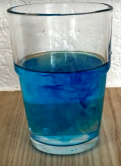
\includegraphics[height=3cm, valign=m]{encre_2}
			\\\hline
			\rotatebox[origin=c]{90}{Micro-état}            &
			
\includegraphics[height=3cm,
			margin=0pt 1ex 0pt 1ex, valign=m]{encre_1_etat} &
			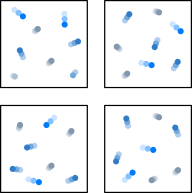
\includegraphics[height=3cm, valign=m]{encre_2_etat}
			\\\hline
		\end{tabularx}
	\end{center}
	\tcblower
	\tcbsubtitle{\fatbox{\textbf{Chauffage d'un corps}}}
	Pour chauffer un corps de manière réversible, il faut donc qu'il n'y ait pas
	de réaction chimique activée par la chaleur, que la température soit
	initialement homogène dans le corps, et que chaque variation soit
	infinitésimale. Ainsi, on peut procéder comme suit~:
	\begin{center}
		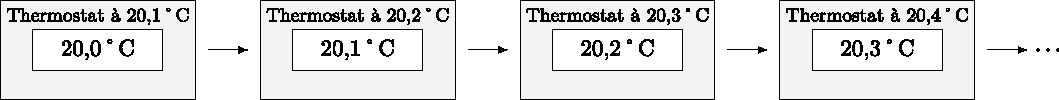
\includegraphics[width=\linewidth]{chauffe_rev}
	\end{center}
\end{tcb}

\vspace{-15pt}
\section{Second principe de la thermodynamique}
\subsection{Énoncé}

\begin{tcb*}(prop){Second ppe.\ de la thermodynamique}
	Il existe une \textbf{fonction d'état}, nommée \textbf{entropie} et notée $S$,
	qui est \textbf{extensive} mais qui \textbf{ne se conserve pas}. Au cours
	d'une transformation d'un système fermé, elle varie selon la loi~:
	\psw{%
		\[
			\boxed{\Delta{S} = S\ind{ech} + S\ind{cr}}
			\Lra
			\boxed{\delta{S} = \delta{S}\ind{ech} + \delta{S}\ind{cr}}
		\]
	}%
	\begin{isd}[sidebyside align=top]
		\vspace{-15pt}
		\tcbsubtitle{\fatbox{\textbf{Entropie échangée}}}
		Pour un système en échangeant de la chaleur avec l'extérieur à $T\ind{ext}$,
		l'entropie échangée est
		\psw{%
			\[
				\delta{S}\ind{ech} = \frac{\delta{Q}}{T\ind{ext}}
				\Lra
				S\ind{ech} = \int_{I}^{F}\frac{\delta{Q}}{T\ind{ext}}
			\]
		}%
		\tcblower
		\vspace{-15pt}
		\tcbsubtitle{\fatbox{\textbf{Entropie créée}}}
		L'entropie créée ne \textbf{peut qu'augmenter}, et on a donc~:
		\smallbreak
		\noindent
		\begin{minipage}[c]{.60\linewidth}
			$\left.
				\parbox{1\linewidth}{%
					\begin{itemize}
						\item[b]{Irréversible}: $\psw{S\ind{cr} > 0}$
						\item[b]{Réversible}: $\psw{S\ind{cr} = 0}$
					\end{itemize}
				}
				\right\}$
		\end{minipage}
		\hfill
		\begin{minipage}[c]{.35\linewidth}
			\hspace{20pt}
			\psw{$S\ind{cr} \geq 0$}
		\end{minipage}
		\vspace{-10pt}
	\end{isd}
\end{tcb*}

Dans l'exemple de chauffage réversible précédent, on pourra montrer en TD que
l'entropie créée est nulle, rendant effectivement la transformation réversible.

\begin{tcb*}(impo){Variation d'entropie}
	L'entropie d'un système \textbf{isolé} tend naturellement vers son
	augmentation, et \textbf{l'entropie créée ne fait qu'augmenter}, par contre
	\textbf{l'entropie d'un système non-isolé peut décroître}~: il est tout à fait
	possible d'avoir $\Delta{S} < 0$ pour un système qui a été «~ordonné~» par un
	autre qui aura alors été «~désordonné~».
\end{tcb*}

\subsection{Cas particuliers}
\begin{tcb*}[label=impl:caspart](impl){Entropie de cas particuliers}
	\begin{itemize}
		\item[b]{Transformation cyclique}: $S$ étant une fonction d'état, on a
		\psw{%
			\[
				\Delta{S}\ind{cycle} = 0
			\]
		}%
		\vspace*{-25pt}
		\item[b]{Transformation adiabatique}: pas d'échange de chaleur, donc
		$\setlength{\fboxsep}{3mm}\boxed{\psw{Q = 0}}$, ainsi
		\psw{%
			\[
				S\ind{ech} = 0
				\quad \Ra \quad
				\boxed{\Delta{S} = S\ind{cr} \geq 0}
			\]
		}%
		\vspace{-20pt}
		\item[b]{Transformation monotherme}: en contact avec un thermostat de
		$T\ind{ext} = T_0 = \cte$, on a
		\psw{%
			\[
				S\ind{ech} = \int_{I}^{F} \frac{\delta{Q}}{T_0} = \frac{Q}{T_0}
			\]
		}%
		C'est également vrai pour les transformations isothermes, qui sont
		forcément monothermes.
		\item[b]{Transformation polytherme}: en contact avec \textbf{plusieurs
			thermostats}, comme $S$ est additive on obtient
		\psw{%
			\[
				S\ind{ech} = \sum_i \frac{Q_i}{T_i}
			\]
		}%
	\end{itemize}
\end{tcb*}

\begin{tcb}(rema)<lftt>{Travail et chaleur}
	On remarque que pour le premier principe, travail et chaleur jouent un rôle
	équivalent. Ça n'est pas le cas pour le second principe. Quand elle a été
	introduite par \textsc{Clausius} en 1864, son but était justement de
	différencier entre \textbf{travail utile ou non}. Un système d'énergie
	«~ordonnée~» va évoluer dans le sens de son désordre, et pas dans le sens
	inverse. Une fois l'état d'\textbf{équilibre atteint}, l'énergie restante est
	sous forme de \textbf{chaleur}, et n'est \textbf{pas utile}, pas récupérable.
	% Dans le cas des frottements,
	% on pourrait les percevoir comme un travail, mais c'est plutôt en termes de
	% chaleur qu'il se conçoivent bien puisque l'énergie échangée n'est \textbf{pas
	% récupérable}.
\end{tcb}

\begin{tcb*}(defi){Transformation isentropique}
	Une transformation est isentropique si l'entropie d'un système ne varie pas au
	cours d'une transformation. Elle doit donc être
	\begin{tasks}[label=\bdmd](2)
		\task \psw{adiabatique}
		\task \psw{réversible}
	\end{tasks}
\end{tcb*}

\section{Expressions de l'entropie}
\begin{tcn}(impo)<itc>{Compétences du programme}
	En MPSI, il ne vous est ni demandé de savoir les démontrer, ni de connaître
	les formules de variation d'entropie. Elles doivent être données, et il faut
	«~juste~» savoir les utiliser.
	% \smallbreak
	% Pour une meilleure compréhension de leur origine, je vous donne les éléments
	% de démonstration ci-après, qui sont donc hors-programme.
\end{tcn}

\subsection{(HP) Définition des grandeurs thermodynamiques}
Dans le premier chapitre, nous avons introduit le concept de grandeur d'état, et
affirmé que seul un petit nombre d'entre elles servaient à décrire le système.
L'entropie d'un système fait partie des grandeurs d'état, et elle se relie aux
autres par les définitions suivantes~:
\begin{tcb}(defi){(HP) Identités thermodynamiques}
	On définit la température et la pression thermodynamiques par~:
	\psw{%
		\[
			T = \eval{\pdv{U}{S}}_{V}
			\qet
			P = -\eval{\pdv{U}{V}}_{S}
		\]
	}%
	On peut alors écrire les fonctions d'état $U$ et $H$ en fonction de $S$, $V$
	et $P$ plutôt que $T$, $V$ et $P$~:
	\smallbreak
	\begin{isd}[sidebyside align=top]
		\tcbsubtitle{\fatbox{\textbf{Première identité}}}
		\psw{%
			\begin{align*}
				\dd{U}         & = \eval{\pdv{U}{S}}_{V}\dd{S} + \eval{\pdv{U}{V}}_{S}\dd{V}
				\\\Lra
				\Aboxed{\dd{U} & = T \dd{S} - P \dd{V}}
			\end{align*}
		}%
		\vspace{-15pt}
		\tcblower
		\tcbsubtitle{\fatbox{\textbf{Seconde identité}}}
		\psw{%
			\begin{align*}
				\dd{H}         & = \dd{U+PV} = \dd{U} + P \dd{V} + V \dd{P}
				\\\Lra
				\Aboxed{\dd{H} & = T \dd{S} + V \dd{P}}
			\end{align*}
		}%
		\vspace{-15pt}
	\end{isd}
	% \begin{itemize}
	% 	\item[b]{Première identité}:
	% 	\psw{%
	% 		\[
	% 			\dd{U} = \eval{\pdv{U}{S}}_{V}\dd{S} + \eval{\pdv{U}{V}}_{S}\dd{V}
	% 			\Lra
	% 			\boxed{\dd{U} = T \dd{S} - P \dd{V}}
	% 		\]
	% 	}%
	% 	\vspace{-15pt}
	% 	\item[b]{Seconde identité}:
	% 	\psw{%
	% 		\[
	% 			\dd{H} = \dd{U+PV} = \dd{U} + P \dd{V} + V \dd{P}
	% 			\Lra
	% 			\boxed{\dd{H} = T \dd{S} + V \dd{P}}
	% 		\]
	% 	}%
	% 	\vspace{-15pt}
	% \end{itemize}
\end{tcb}

\begin{tcb}(rema)<lftt>{Correspondances entre définitions}
	Ces grandeurs définies grâce à des outils thermodynamiques sont identifiées à
	celles construites à partir de la théorie cinétique.
\end{tcb}

\begin{tcb}[label=prop:dS, sidebyside](prop){(HP)
			Expression infinitésimale de la variation d'entropie}
	\tcbsubtitle{\fatbox{\textbf{Première identité}}}
	\psw{%
		\begin{align*}
			\dd{S}    & = \frac{\dd{U}}{T} + P \frac{\dd{V}}{T}
			\\\Lra
			\Delta{S} & = \int_{I}^{F} \frac{\dd{U}}{T} + P \frac{\dd{V}}{T}
		\end{align*}
	}%
	\vspace{-15pt}
	\tcblower
	\tcbsubtitle{\fatbox{\textbf{Seconde identité}}}
	\psw{%
		\begin{align*}
			\dd{S}    & = \frac{\dd{H}}{T} - V \frac{\dd{P}}{T}
			\\\Lra
			\Delta{S} & = \int_{I}^{F} \frac{\dd{H}}{T} - V \frac{\dd{P}}{T}
		\end{align*}
	}%
	\vspace{-15pt}
\end{tcb}

\subsection{Phases condensées}
\begin{tcbraster}[raster equal height=rows, raster columns=2]
	\begin{tcb*}(prop){$\Delta{S}\sup{cond}$}
		L'entropie d'une masse $m$ d'une phase condensée ne dépend que
		de la température, et on a
		\psw{%
			\[
				S(T) = mc \ln \frac{T}{T\ind{ref}} + S\ind{ref}
				\boxed{\Delta{S} = mc \ln \frac{T_f}{T_i}}
			\]
		}%
		\vspace{-15pt}
	\end{tcb*}
	\begin{tcb}(demo)'r'{(HP) $\Delta{S}\sup{cond}$}
		On a $\dd{V} = 0$, donc d'après l'expression de l'entropie
		(Propriété~\ref{prop:dS})~:
		\psw{%
			\begin{align*}
				% \Delta{S}\sup{cond} & = \int_{I}^{F} \frac{\dd{U}}{T} + 0
				% \\\Lra
				\Delta{S}\sup{cond} & = C_V \int_{I}^{F} \frac{\dd{T}}{T}
				\\\Lra
				\Delta{S}\sup{cond} & = mc \ln \frac{T_f}{T_i}
				\qed
			\end{align*}
		}%
		\vspace{-15pt}
	\end{tcb}
\end{tcbraster}

\begin{tcb*}[breakable](appl)<lftt>{Entropie d'un mélange}
	On peut vérifier avec cette expression que l'état final d'un mélange
	correspond bien au maximum de l'entropie du système.
	\smallbreak
	On mélange $m = \SI{300}{g}$ d'eau à $T_{i,1} = \SI{50}{\degreeCelsius}$ et
	$m = \SI{300}{g}$ d'eau à $T_{i,2} = \SI{20}{\degreeCelsius}$ dans un
	calorimètre. On le suppose parfaitement calorifugé, et on néglige pour
	simplifier sa capacité calorifique.
	\smallbreak
	On donne $\Delta{S} = mc \ln \frac{T_f}{T_i}$ la variation d'entropie d'une
	phase condensée. On note $T_1$ et $T_2$ la température des masses d'eau
	\textbf{hors équilibre}.
	\begin{enumerate}[label=\sqenumi]
		\item Faire un bilan d'enthalpie pour trouver l'expression littérale et
		      la valeur numérique de $\Delta{H}$. En déduire $T_2$ en fonction de
		      $T_{i,2}$, $T_{i,1}$ et $T_1$.
		\item Exprimer la variation d'entropie du système en éliminant
		      l'expression de $T_2$ par le résultat précédent. En déduire
		      l'expression de l'entropie créée $S\ind{cr}$, puis la tracer en
		      fonction de $T_1$. Conclure.
	\end{enumerate}
	\tcblower
	\begin{enumerate}[label=\sqenumi]
		\item[m]
			\psw{%
				\begin{DispWithArrows*}
					\Delta{H} &= mc\ind{eau} (T_2 - T_{i,2}) + mc\ind{eau} (T_1 - T_{i,1})
					\Arrow{$\Delta{H} = Q$\\$Q = 0$}
					\\\Lra
					0 &= \cancel{mc\ind{eau}} (T_2 - T_{i,2} + T_1 - T_{i,1})
					\\\Lra
					\Aboxed{T_2 &= T_{i,2} + T_{i,1} - T_1}
				\end{DispWithArrows*}
			}%
		\item \vspace{-15pt}
		      \noindent
		      \begin{minipage}[t]{.60\linewidth}
			      \psw{%
				      \begin{DispWithArrows*}[]
					      \Delta{S} &=
					      mc \ln (\frac{T_2}{T_{i,2}}) + mc \ln (\frac{T_1}{T_{i,1}})
					      \\\Lra
					      \Delta{S} &=
					      mc \ln (\frac{T_{i,2} + T_{i,1} - T_1}{T_{i,2}}) +
					      mc \ln (\frac{T_1}{T_{i,1}})
					      % \Arrow{$Q = 0 \Ra S\ind{ech} = 0$}
					      \\\Lra
					      \Aboxed{
						      S\ind{cr} &=
						      mc \ln (\frac{T_{i,2} + T_{i,1} - T_1}{T_{i,2}}) +
						      mc \ln (\frac{T_1}{T_{i,1}})
					      }
				      \end{DispWithArrows*}
			      }%
		      \end{minipage}
		      \hfill
		      \begin{minipage}[t]{.40\linewidth}
			      \vspace{0pt}
			      \begin{center}
				      \sswitch{
					      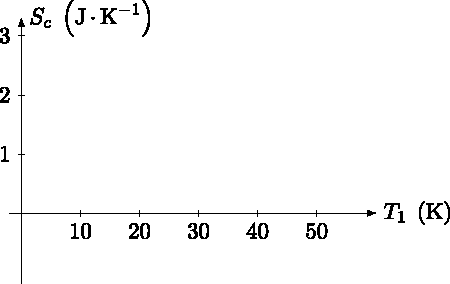
\includegraphics[width=\linewidth]{calo_Smax-stud}
				      }{
					      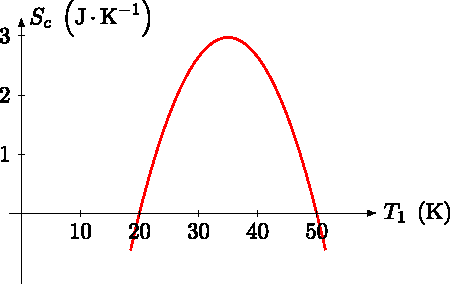
\includegraphics[width=\linewidth]{calo_Smax}
				      }
			      \end{center}
		      \end{minipage}
	\end{enumerate}
	\textbf{Conclusion~:} \psw{La température d'équilibre $T_f =
			\SI{35}{\degreeCelsius}$ correspond au maximum de $S_c$}
\end{tcb*}

\vspace{-15pt}
\subsection{Gaz parfait}
\begin{tcbraster}[raster equal height=rows, raster columns=2]
	\begin{tcb*}(prop){$\Delta{S}\sup{G.P.}$}
		L'entropie d'un gaz parfait caractérisé par $(P,V,T)$ peut s'exprimer avec
		différentes variables, par exemple
		\psw{%
			\[
				S(T,V) =
				C_V \ln (\frac{T}{T\ind{ref}}) + nR \ln (\frac{V}{V\ind{ref}}) +
				S\ind{ref}
			\]
		}%
		et sa variation peut s'écrire de trois manières différentes~:
		\psw{%
			\begin{align*}
				\Delta{S} & = C_V \ln (\frac{T_f}{T_i}) + nR \ln (\frac{V_f}{V_i})
				\\\Lra
				\Delta{S} & = C_P \ln (\frac{T_f}{T_i}) - nR \ln (\frac{P_f}{P_i})
				\\\Lra
				\Delta{S} & = C_V \ln (\frac{P_f}{P_i}) + C_P \ln (\frac{V_f}{V_i})
			\end{align*}
		}%
		\vspace{-15pt}
	\end{tcb*}
	\begin{tcb}(demo)'r'{(HP) $\Delta{S}\sup{G.P.}$}
		D'après l'expression de l'entropie \textit{via} la première identité
		(Propriété~\ref{prop:dS})~:
		\psw{%
			\begin{align*}
				\Delta{S}\sup{G.P.} & = \int_{I}^{F} \frac{C_V\dd{T}}{T} + \frac{P
					\dd{V}}{T}
				\\\Lra
				\Delta{S}\sup{G.P.} & = C_V \ln \frac{T_f}{T_i} + \int_{I}^{F} nR
				\frac{\dd{V}}{V}
				\\\Lra
				\Delta{S}\sup{G.P.} & = C_V \ln \frac{T_f}{T_i} + nR \ln \frac{V_f}{V_i}
				\qed
			\end{align*}
		}%
		On trouve la deuxième formule avec la seconde identité, et la troisième en
		utilisant l'équation d'état du gaz parfait.
	\end{tcb}
\end{tcbraster}

\subsection{Loi de \textsc{Laplace}}
En combinant les expressions précédentes et en les appliquant à des
transformations isentropiques, on obtient les lois de \textsc{Laplace}~:

\begin{tcbraster}[raster equal height=rows, raster columns=3]
	\begin{tcb*}[raster multicolumn=2](prop){Loi de \textsc{Laplace}}
		Pour une transformation \textbf{adiabatique} et \textbf{réversible} d'un
		\textbf{gaz parfait}, les paramètres d'état sont reliés par les relations
		suivantes~:
		\psw{%
		\[
			PV^{\gamma} = \cte
			\qou
			P^{1-\gamma}T^{\gamma} = \cte
			\qou
			TV^{\gamma-1} = \cte
		\]
		}%
		où $\gamma > 1$ est le coefficient adiabatique du fluide.
	\end{tcb*}
	\begin{tcb*}[list entry={\lte Loi de \textsc{Laplace}}](impo)'r'{}
		Il est nécessaire de \textbf{connaître} et \textbf{citer} les
		conditions d'applications~:
		\begin{tasks}[label=\bdmd]
			\task \psw{Adiabatique $Q=0$~;}
			\task \psw{Réversible~;}
			\task \psw{Gaz parfait.}
		\end{tasks}
	\end{tcb*}
\end{tcbraster}

\begin{tcb*}(demo){Loi de \textsc{Laplace}}
	\psw{%
		\begin{DispWithArrows*}[]
			\Delta{S} &= C_V \left(\ln (\frac{P_f}{P_i}) + \frac{C_P}{C_V} \ln
				(\frac{V_f}{V_i})\right)
			\Arrow{$\gamma = C_P/C_V$}
			\\\Lra
			\Delta{S} &= C_V \left(\ln (\frac{P_f}{P_i}) + \gamma \ln
				(\frac{V_f}{V_i})\right)
			\Arrow{$a \ln b = \ln b^a$\\$\ln a + \ln c = \ln ac$}
			\\\Lra
			\Delta{S} &= C_V \ln (\frac{P_fV_f^{\gamma}}{P_iV_i^{\gamma}})
			\Arrow{Adiabatique réversible\\$\Ra \Delta{S} = 0$}
			\\\Lra
			1 &= \frac{P_fV_f^{\gamma}}{P_iV_i^{\gamma}}
			\qed
		\end{DispWithArrows*}
	}%
	On retrouve les autres formes par l'équation d'état du gaz parfait à partir de
	ce résultat, ou les démontrer à partir des autres formules et des expressions
	de $C_V$ et $C_P$ en fonction de $\gamma$~:
	\[
		\psw{C_V = \frac{nR}{\gamma-1}}
		\qet
		\psw{C_P = \frac{\gamma nR}{\gamma-1}}
	\]
\end{tcb*}

\section{Applications}
\subsection{Méthode de bilans d'entropie}
\begin{tcb*}(ror){Bilans d'entropie}
	\begin{enumerate}[label=\sqenumi]
		\item Modéliser le système~: gaz parfait ou phase condensée~?
		\item Calculer la variation totale d'entropie avec la formule pertinente~;
		\item Calculer l'entropie échangée $S\ind{ech}$ selon les conditions
		      extérieures (voir Cas particuliers~\ref{impl:caspart}), en général
		      $S\ind{ech} = \int_{I}^{F} \frac{\delta{Q}}{T\ind{ext}}$~;
		\item Calculer l'entropie créée par $S\ind{cr} = \Delta{S} - S\ind{cr}$~;
		\item Conclure quant à la nature réversible ($S\ind{cr} = 0$) ou
		      irréversible ($S\ind{cr} > 0$) de la transformation.
	\end{enumerate}
\end{tcb*}

\subsection{Transformation isochore et monotherme d'un gaz parfait}
\begin{tcb*}[breakable](appl)<lftt>{Transfo$^\circ$ isoV.\ et monoT.\ d'un G.P.}
	Soit un gaz parfait passant de l'état initial $I$ $(T_i, P_i, V_i = V_0)$ à
	un état final $f$ $(T_f, P_f, V_f = V_0)$ en le mettant en contact avec un
	thermostat de température $T\ind{ext} = T_f$.
	\begin{enumerate}[label=\sqenumi]
		\item Déterminer la variation d'entropie totale en fonction de $n$, $R$,
		      $\gamma$, $T_f$ et $T_i$
		\item Déterminer l'entropie échangée en fonction des mêmes variables.
		\item Déterminer l'entropie créée, et tracer l'expression obtenue avec $x
			      = \frac{T_i}{T_f}$. Conclure sur la nature réversible ou non de la
		      transformation.
		\item Reprendre les questions pour une transformation \textbf{isobare} et
		      monotherme.
	\end{enumerate}
	\tcblower
	\begin{enumerate}[label=\sqenumi]
		\item[m][30]
		\psw{%
			\begin{gather*}
				\Delta{S} =
				C_V \ln \frac{T_f}{T_i} +
				\underbracket[1pt]{nR \ln \frac{V_f}{V_i}}_{=0}
				\Ra
				\boxed{\Delta{S} = \frac{nR}{\gamma-1} \ln (\frac{T_f}{T_i})}
			\end{gather*}
		}%
		\vspace{-20pt}
		\item[m][30]
		\psw{%
			\begin{align*}
				\beforetext{Transformation monotherme donc}
				S\ind{ech}                   & = \frac{Q}{T_f}
				\\\beforetext{Transformation isochore donc}
				\Delta{U}                    & = Q + \cancel{W}
				\\\beforetext{Première loi de \textsc{Joule}}
				\Lra
				\frac{nR}{\gamma-1}(T_f-T_i) & = Q
				\\\beforetext{On combine}
				\Ra
				\Aboxed{
				S\ind{ech}                   & =
					\frac{nR}{\gamma-1} \left(1 - \frac{T_i}{T_f}\right)
				}
			\end{align*}
		}%
		\item ~
		      \smallbreak
		      \begin{isd}
			      \psw{%
				      \begin{align*}
					      \Delta{S} & = S\ind{ech} + S\ind{cr}
					      \\\Lra
					      S\ind{cr} & =
					      \frac{nR}{\gamma-1} \ln (\frac{T_f}{T_i}) -
					      \frac{nR}{\gamma-1} \left(1 - \frac{T_i}{T_f}\right)
					      \\\Lra
					      \Aboxed{
					      S\ind{cr} & =
						      \frac{nR}{\gamma-1}
						      \left( \frac{T_i}{T_f} - 1 - \ln \frac{T_i}{T_f} \right)
					      }
					      \\\Lra
					      S\ind{cr} & = C_V (x - 1 - \ln x)
				      \end{align*}
			      }%
			      \tcblower
			      \begin{center}
				      \sswitch{
					      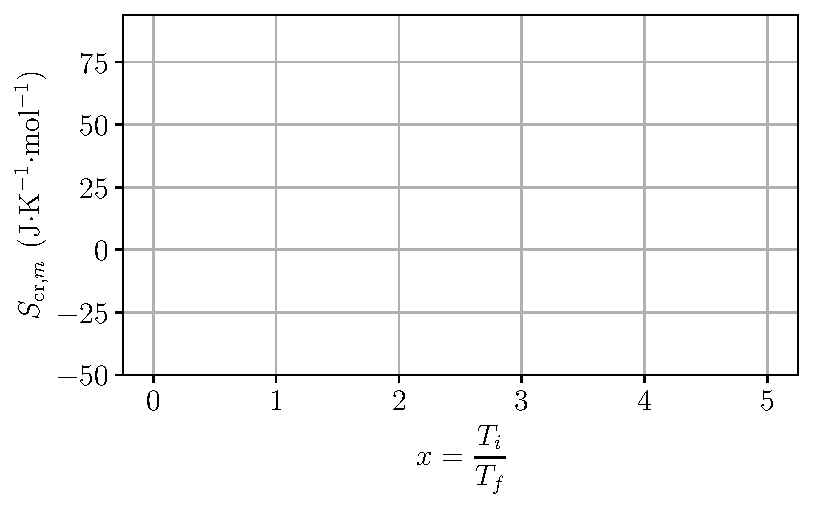
\includegraphics[width=\linewidth]{DSappl_1-stud}
				      }{
					      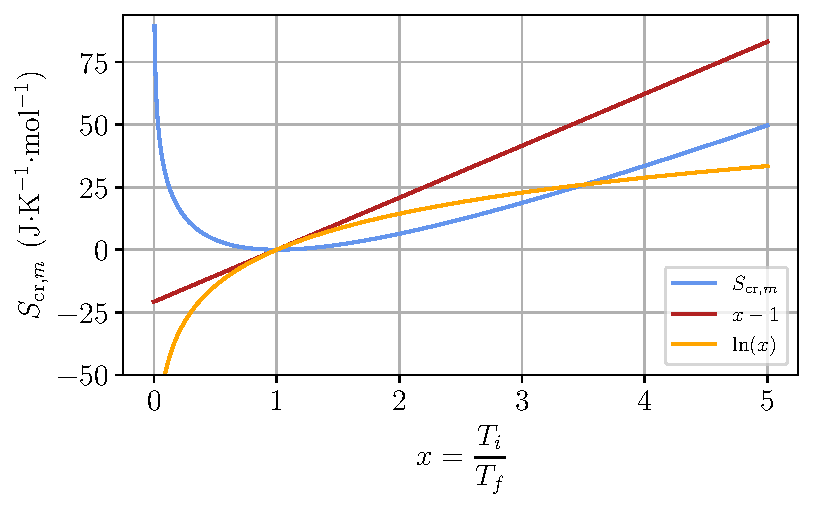
\includegraphics[width=\linewidth]{DSappl_1}
				      }
			      \end{center}
		      \end{isd}
		      \textbf{Conclusion}~: \psw{l'entropie créée est \textbf{positive} pour
			      $T_f \neq T_i$~: c'est une transformation irréversible.}
		\item[m]
			\everymath{\sswitch{\color{white}}{\color{\mycol}}}
			\begin{align*}
				\Delta{S}                           & =
				C_P \ln \frac{T_f}{T_i} -
				\underbracket[1pt]{nR \ln \frac{P_f}{P_i}}_{=0}
				\\\Ra
				\Aboxed{
				\Delta{S}                           & = \frac{\gamma nR}{\gamma-1} \ln (\frac{T_f}{T_i})
				}
				\\
				\beforetext{Transformation monotherme}
				S\ind{ech}                          & = \frac{Q}{T_f}
				\\\beforetext{Transformation isobare}
				\Delta{H}                           & = Q + \cancel{W_u}
				\\\beforetext{Loi de \textsc{Joule}}
				\Lra
				\frac{\gamma nR}{\gamma-1}(T_f-T_i) & = Q
				\\\beforetext{On combine}
				\Ra
				\Aboxed{
				S\ind{ech}                          & =
					\frac{\gamma nR}{\gamma-1} \left(1 - \frac{T_i}{T_f}\right)
				}
				\\\beforetext{Second principe}
				\Delta{S}                           & = S\ind{ech} + S\ind{cr}
				\\\Lra
				S\ind{cr}                           & =
				\frac{nR}{\gamma-1} \ln (\frac{T_f}{T_i}) -
				\frac{nR}{\gamma-1} \left(1 - \frac{T_i}{T_f}\right)
				\\\Lra
				\Aboxed{
				S\ind{cr}                           & =
					\frac{nR}{\gamma-1}
					\left( \frac{T_i}{T_f} - 1 - \ln \frac{T_i}{T_f} \right)
				}
				\\\Lra
				S\ind{cr}                           & = C_V (x - 1 - \ln x)
			\end{align*}
	\end{enumerate}
\end{tcb*}

\end{document}
